%--------------------------------------------------------------
% thesis.tex 
%--------------------------------------------------------------
% - template for the main file of Informatica@Unifi Thesis 
% - based on Classic Thesis Style Copyright (C) 2008 
%   Andr\'e Miede http://www.miede.de   
%--------------------------------------------------------------

%--------------------DOCUMENT-CLASS----------------------------
%\documentclass[openright,titlepage,oneside,fleqn,
%	headinclude,12pt,a4paper,footinclude,makeidx]{scrbook}
\documentclass[openright,titlepage,oneside,fleqn,
	headinclude,12pt,a4paper,footinclude,makeidx]{scrbook}

% sostituire "oneside" con "twoside" per stampa fronte-retro
% aggiungere "hidelinks" per eliminare i box nei link ipertestuali
%--------------------------------------------------------------

%--------------------PACKAGES----------------------------------
\usepackage[italian]{babel} % italian rende i nomi "bibliography" e "index" in italiano
\usepackage[fixlanguage]{babelbib} % per creare la bibliografia in lingua
\usepackage[utf8]{inputenc} 
%\usepackage{lmodern}
\usepackage[T1]{fontenc} 
%\usepackage{textcomp}
%\usepackage[OT1]{fontenc}
\usepackage[square,numbers]{natbib} 
\usepackage[fleqn]{amsmath}
\usepackage{amssymb}
\usepackage{ellipsis}
\usepackage{listings}
\usepackage{lstautogobble}
\usepackage{subfig}
\usepackage[format=plain,labelformat=simple,labelsep=colon]{caption}
\usepackage{appendix}
\usepackage{siunitx}
\usepackage{lipsum}
\usepackage{multirow} % per tabelle multirow
\usepackage{comment} % per enviroment comment: \begin{comment}...\end{comment}
\usepackage{dia-classicthesis-ldpkg}

\usepackage{amsthm} %necessaria per theoremstyle
\usepackage{mathabx} %per bigtimes, simbolo di prodotto cartesiano


\usepackage[eulerchapternumbers, linedheaders, subfig, beramono, eulermath, parts, dottedtoc]{classicthesis}
% Se non usiamo dottedtoc per l'indice,
% \usepackage[eulerchapternumbers,linedheaders,subfig,beramono,eulermath, parts]{classicthesis}
% al suo posto usiamo tocstyle:
% \usepackage{tocstyle}
% \usetocstyle{allwithdot}
% PROBLEMA: nome dei capitoli minuscoli
%\renewcommand{\cftchappagefont}{\normalfont}
%\usepackage{tocloft}
%\renewcommand{\cfttoctitlefont}{\hfill\Large\itshape}
%\renewcommand\cfttocfont{\normalfont}

\usepackage{imakeidx}
\makeindex[intoc] % aggiunge al ToC l'indice analitico
% sembra non funzionare con tocstyle
%\makeindex

\usepackage{wrapfig}
\usepackage[italian,noabbrev]{cleveref}
%---------------------------------------------------------------

%--------------------NEWCOMMANDS--------------------------------
\newcommand{\myItalianTitle}{L'influenza della percezione del rischio nelle dinamiche epidemiche: un approccio con la modellizzazione ad agenti\xspace}
\newcommand{\myEnglishTitle}{Influence of risk perception in epidemic spreading: an agent-based approach\xspace}
\newcommand{\myDegree}{Corso di Laurea in Fisica e Astrofisica\xspace}
\newcommand{\myCurriculum}{Generale\xspace}
\newcommand{\myName}{Giulia Leone\xspace}
\newcommand{\myRelatore}{Franco Bagnoli\xspace}
%\newcommand{\myCorelatore}{Gabriele Costa\xspace}
%\newcommand{\myOtherCorelatore}{Letterio Galletta\xspace}
\newcommand{\myFaculty}{Scuola di Scienze Matematiche, Fisiche e Naturali\xspace}
\newcommand{\myUni}{\protect{Università degli Studi di Firenze}\xspace}
\newcommand{\myLocation}{Firenze\xspace}
\newcommand{\myTime}{Anno Accademico 2019-2020\xspace}

% \newcommand{\myVersion}{Version 0.1\xspace} % mi dice already defined
% \renewcommand{\myVersion}{Version 0.1\xspace} % forza, ma tempo potrebbe creare conflitti
\newcommand{\myVersione}{Versione 1.0.1\xspace}


% Diritto d'autore: Attribution-NonCommercial-ShareAlike 4.0 International 
% \newcommand{\mycopyright}{
\includegraphics[width=1.5cm]{1-front/copyright/by-nc-sa.png} 
%	\href{https://creativecommons.org/licenses/by-nc-sa/4.0/}{Creative
%		Commons Attribution-NonCommercial-ShareAlike 4.0 International (CC BY-NC-SA 4.0)  }\xspace}

% Diritto d'autore: Attribution-NonCommercial-NoDerivatives 4.0 International
% \newcommand{\mycopyright}{
\includegraphics[width=1.5cm]{1-front/copyright/by-nc-nd.png} 
%	\href{https://creativecommons.org/licenses/by-nc-nd/4.0/}{Creative
%		Commons Attribution-NonCommercial-NoDerivatives 4.0 International (CC BY-NC-ND 4.0) }\xspace}

%\newcommand{\mycopyright}{\includegraphics{1-front/copyright/by-nc-sa-compact.png} 
%	\href{https://creativecommons.org/licenses/by-nc-sa/4.0/}{Creative
%		Commons Attribution - NonCommercial - ShareAlike 4.0 International (CC BY-NC-SA 4.0)  }\xspace}
		
\newcommand{\mycopyright}{%
\includegraphics[width=0.3cm]{front/copyright/c.png} 
\textcopyright\ \xspace}

%\newcommand{\disps}{dispositivo crittografico }
%\newcommand{\dispp}{dispositivi crittografici }


%\newcommand{\codice}[4]
%{\begin{center}
%\lstinputlisting[language={C},firstline={#1}, lastline={#2},caption={#3},label={#4}]{"D:/UNIFI/Magistrale/Tesi/spectre/primeProbe/spark.c"}
%\end{center}}
	
%\newcommand{\codspark}[3]{
%\begin{center}
%\lstinputlisting[language={C},firstline={#1},lastline={#2},firstnumber={#1},caption={[#3]}]{other/code/spark.c}
%\end{center}}

\newcommand{\arr}[2]{$\text{\texttt{#1}}\left[ \text{\texttt{#2}}\right]$}
\newcommand{\arrdoppio}[3]{$\text{\texttt{#1}}\left[ \text{\texttt{#2}} \left[\text{\texttt{#3}}\right]\right]$}

% \newcommand{\kilobyte}{kB}
% \newcommand{\megabyte}{MB}
% \newcommand{\gigahertz}{GHz}

\newcommand{\tcal}{\mathbb{T}}
\newcommand{\talfa}{\mathbb{T}_{\alpha}}
\newcommand{\tbeta}{\mathbb{T}_{\beta}}

\newcommand{\myfloatalign}{\centering}
% how all the floats will be aligned

\renewcommand{\lstlistingname}{Codice}% Listing -> Codice
\renewcommand{\lstlistlistingname}{Elenco dei Codici}% Listings -> List of Algorithms

\theoremstyle{plain}
\newtheorem{teorema}{Teorema}[chapter]
\theoremstyle{definition}
\newtheorem{definizione}{Definizione}[chapter]
\theoremstyle{definition}
\newtheorem{esempio}{Esempio}[chapter]
%\theoremstyle{plain}
%\newtheorem{corollario}{Corollario}[teorema]
%\theoremstyle{plain}
%\newtheorem{proposizione}{Proposizione}[teorema]
%\theoremstyle{definition}
%\newtheorem{protocollo}{Protocollo}[chapter]
%\newenvironment{sistema}%
%	{\left\lbrace\begin{array}{@{}l@{}}}%
%	{\end{array}\right.}
%--------------------------------------------------------------

%--------------------SETTINGS----------------------------------
\newlength{\abcd} % for ab..z string length calculation
\setlength{\extrarowheight}{3pt} % increase table row height
\captionsetup{format=hang,font=small}

\graphicspath{{other/img/}}

\crefname{listing}{codice}{codici}

% Layout settings
\usepackage{geometry}
\geometry{
	a4paper,
	ignoremp,
	bindingoffset = 1cm, 
	textwidth     = 13.5cm,
	textheight    = 21.5cm,
	lmargin       = 3.5cm, % left margin
	tmargin       = 4cm    % top margin 
}

\lstset{ %
	basicstyle=\small\ttfamily, 		% the size of the fonts that are used for the code
	breaklines=true,                	% sets automatic line breaking
	captionpos=b,                   	% sets the caption-position to bottom
	commentstyle=\color{violet},   		% comment style
	frame=none,							% adds a frame around the code
	frameround=fttt,					% round corner (use f instead t to edge corner)
	keepspaces=true,                	% keeps spaces in text, useful for keeping indentation of code (possibly needs columns=flexible)
	keywordstyle=\color{blue},      	% keyword style
	language=C,               			% the language of the code
	numbers=left,                   	% where to put the line-numbers; possible values are (none, left, right)
	numbersep=5pt,                  	% how far the line-numbers are from the code
	numberstyle=\scriptsize\color{black}, % the style that is used for the line-numbers
	stepnumber=1,                   	% the step between two line-numbers. If it's 1, each line will be numbered
	stringstyle=\color{Brown},  		% string literal style
	tabsize=2                   		% sets default tabsize to 2 spaces
}

\lstdefinelanguage{NetLogo}{
    breaklines=true,
    breakatwhitespace=true,
    alsoletter={-,?,.},
    morekeywords=[1]{turtles-own, to, to-report, end},
    keywordstyle=[1]\color[rgb]{0.25,0.5,0.35},
    morekeywords=[2]{ask, let, set, if, report, ifelse,  clear-all, no-display, set-default-shape, create-turtles, fd, create-link-with, repeat, display, reset-ticks, stop, create-turtle, move-to, tick, facexy, layout-spring},
    keywordstyle=[2]\color{blue},
    morekeywords=[3]{turtles, count, with, out-link-neighbors, random-float, exp, not, n-of, color, any?, size, sqrt, my-links, one-of, both-ends, of, links, distancexy},
    keywordstyle=[3]\color[rgb]{0.6,0,0.8},
    comment=[l]{\;},
    commentstyle=\color[rgb]{0.5,0.5,0.5},
    string=[d]{"},
    stringstyle=\color{orange},
    morekeywords=[4]{red, green, yellow, true, false},
    keywordstyle=[4]{\color{orange}},
    %numberstyle={\color{orange}},
}
%--------------------PARAMETERS-------------------------------
\begin{document}
\frenchspacing
\raggedbottom
%--------------------------------------------------------------

%---------------------FRONTMATTER------------------------------
% A book’s front matter contains such things as the title page, an abstract, a table of contents, a preface, a list of notations, a list of figures, and a list of tables. Some of these front matter pages, such as the title page, are traditionally not numbered.

% The \frontmatter declaration makes the pages numbered in lowercase roman, and makes chapters not numbered, although each chapter’s title appears in the table of contents;
% \pagenumbering{roman} %_scambiare i due seguenti comandi con \frontmatter
% \pagestyle{plain} 
% se usiamo \frontmatter, i comandi soprastanti non sono necessari
\frontmatter 

% Pagina di Titolo
%--------------------------------------------------------------
% titlepage.tex (use thesis.tex as main file)
%--------------------------------------------------------------
\begin{titlepage}
	\begin{center}
   	\large
      \hfill
      \vfill
      \begingroup
         
\includegraphics[scale=0.15]{1-front/logo/LOGO}\\
%\left 			\spacedallcaps{\myUni} \\ 
			\myFaculty \\
			\vspace{0.5cm}
			\myDegree \\ 
			%Curriculum: \emph{\myCurriculum}\\
			%\vspace{0.5cm}
         \vspace{0.5cm}    
         Tesi di Laurea 
      \endgroup 
      \vfill 
      \begingroup
      	\color{Maroon}\spacedallcaps{\myItalianTitle} \\ $\ $\\
      	\spacedallcaps{\myEnglishTitle} \\ 	
	\bigskip
      \endgroup
      \spacedlowsmallcaps{\myName}
      \vfill 
      \vfill
      Relatore: Prof. \emph{\myRelatore}\\
      %Corelatori: Dott. \emph{\myCorelatore}, Dott. \emph{\myOtherCorelatore}
      \vfill
      \vfill
      \myTime
      \vfill                      
	\end{center}        
\end{titlepage}   
%--------------------------------------------------------------
% back titlepage
%--------------------------------------------------------------
   \newpage
	\thispagestyle{empty}
	\hfill
	\vfill
	\noindent\myName: 
	\textit{\myItalianTitle,} 
	\myVersione,
	\myDegree, \mycopyright, \myUni, \myTime
%--------------------------------------------------------------
% back titlepage end
%--------------------------------------------------------------

% Dedica
%\thispagestyle{empty}
\begin{flushright}
\textit{A <Nome>, \\
frase di dedica.}
\end{flushright}

%\newpage
\bigskip

\thispagestyle{empty}
\begin{flushright}
\textit{"Citazione coltissima"} \textit{Autore, "Titolo", 19xx, rif bibliografia.}
\end{flushright}


\pagestyle{scrheadings}
% the page number jumps to the header (in alto a destra).
 
% \pagenumbering{arabic} 
% usare qui, se si desidera numerazione araba unica delle pagine
% spostare in mainmatter, se vogliamo numerazione romana per front e araba per il resto

% ToC
\tableofcontents

%% Elenco Immagini
%\listoffigures
%
%% Elenco Codici
%\lstlistoflistings
%
%% Elenco Tabelle
%\begingroup
%\let\clearpage\relax
%\let\cleardoublepage\relax
%\let\cleardoublepage\relax
%\vspace*{8ex}
%\listoftables
%\endgroup 

% Citazione
\cleardoublepage
\thispagestyle{empty}
\thispagestyle{empty}
\begin{flushright}
\null\vspace{\stretch {1}}
\emph{"Citazione colta,\\ma colta colta,\\in italiano."\\} 
\null\vspace{5mm}
\emph{"Citazione colta,\\ma colta colta,\\in inglese." \break --- Opera, Autore} \vspace{\stretch{2}}\null
\end{flushright}
\cleardoublepage

%--------------------------------------------------------------

%---------------------MAINMATTER-------------------------------

% The \mainmatter changes the behavior back to the expected version, and resets the page number
\mainmatter
%\pagenumbering{arabic}
% use \cleardoublepage here to avoid problems with pdfbookmark
% il comando sottostante elimina le pagine bianche tra un cap e l'altro
% consiglio l'eliminazione per la stampa fronte retro => cap iniziano sempre sulla pagine destra
% \let\cleardoublepage\clearpage	
% \include{intro} % use \myChapter command instead of \chapter
% \cleardoublepage\myPart{Part I}
% \cleardoublepage\myPart{Part II}

% Capitoli
\addcontentsline{toc}{chapter}{Introduzione}
\chapter*{Introduzione} \markboth{}{Introduzione}
% l'uso di '*' rende il capitolo non numerato ed indicizzato nel toc
% lo aggiungiamo noi al toc tramita la prima istruzione
% con \markboth{<left output>{<right output>} evitiamo che nell'header compaia il titolo del capitolo precedente

%\chapter{Introduzione}
\label{chap:intro}
Mai quanto nel corso degli ultimi mesi si è mantenuta alta l'attenzione sul problema della diffusione di un'infezione; se prima erano ad appannaggio quasi esclusivo degli addetti al settore, chiunque di noi, oggi, ha certamente consultato almeno una volta mappe e grafici per provare a comprendere cosa stesse succedendo o per orientarsi fra i numeri comunicati giornalmente dai mezzi di informazione. In questo contesto, la modellazione epidemica riveste un ruolo essenziale, in quanto uno dei suoi primi propositi è proprio quello di riuscire a descrivere in modo minuzioso le modalità in cui un virus viene trasmesso da un individuo all'altro; inoltre, permette di gettare uno sguardo a quelli che potrebbero essere gli sviluppi futuri di un'epidemia e di reagire il più prontamente possibile al suo dilagare. 
\\Partendo dal modello di epidemia su rete sviluppato da Bagnoli \textit{et al.} in \cite{Bagnoli2014}, quello che ci siamo proposti di fare in questo lavoro di tesi è valutare come la propagazione di una malattia infettiva venga influenzata da una diversa percezione del rischio dei componenti della rete, obiettivo che ci siamo prefissati di raggiungere con l'ausilio di un approccio ad agenti. L'elaborato è suddiviso in quattro capitoli, il cui contenuto viene qui esposto brevemente:
\begin{itemize}
\item \textit{Capitolo 1}: si descrive cosa significhi modellare un'epidemia, con particolare attenzione a quali siano gli obiettivi che si intende raggiungere e, al contempo, i limiti che si incontrano nel perseguire questo intento. Dopo aver fatto cenno all'approccio compartimentale, si esplora il modello SIR e si mette in rilievo l'importanza del numero di riproduzione di base $\mathcal{R}_0$; infine, si dedica spazio alla modellizzazione ad agenti, che annovera fra i suoi pregi la capacità di evidenziare l'emergenza di tutta una serie di comportamenti collettivi che altrimenti non potrebbero venire predetti.
\item \textit{Capitolo 2}: si introducono una serie di concetti teorici legati ai grafi, concetti che saranno utili per meglio descrivere l'andamento di un'epidemia su rete.
\item \textit{Capitolo 3}: si tratta della percezione del rischio e della sua influenza sull'andamento della diffusione dell'infezione; questo elemento viene matematicamente formalizzato andando a modificare la probabilità netta di contrarre la malattia mediante l'aggiunta di due fattori, il primo basato sulla frazione di contatti infetti e l'altro relativo alle misure precauzionali che possono essere messe in atto. Si esplora l'andamento dell'epidemia su due diversi tipi di rete (poissoniana e scale-free) e se ne riportano i risultati sperimentali ottenuti in \cite{Bagnoli2007} e in \cite{Bagnoli2014}.
\item \textit{Capitolo 4}: facendo riferimento ai concetti introdotti e ai risultati evidenziati nei capitoli precedenti, si spiega come sia stato costruito il modello NetLogo del quale ci si è serviti per condurre le simulazioni; se ne sono poi messi in luce gli esiti e il loro confermare quanto precedentemente ottenuto.
\end{itemize}

\chapter{Titolo del primo capitolo}
\label{chap:cap1}
L'obiettivo dietro alla creazione di un modello matematico di una malattia infettiva è quello di arrivare a comprenderne e a descriverne il processo di trasmissione. In linea del tutto generale, possiamo andare a semplificarlo come segue:
%\begin{enumerate}
%\item \textit{a.} in primo luogo, uno o più soggetti infetti vengono introdotti in una popolazione di individui suscettibili (a rischio, cioè, di contrarre la malattia);
%\item \textit{b.} un individuo che viene infettato può inizialmente rimanere asintomatico, per poi mostrare i sintomi; può guarire, sia grazie all'assunzione di medicinali che all'azione del sistema immunitario, ed acquisire così una protezione nei confronti di una possibile reinfezione;
%\item \textit{c.} quando il bacino dei potenziali suscettibili viene sufficientemente svuotato, la diffusione inizia a rallentare fino a fermarsi; se vengono aggiunti nuovi soggetti alla popolazione, che sia a seguito di flussi migratori o di nascite, l'epidemia può persistere per un lungo periodo di tempo e diventare così endemica. \\
%\end{enumerate}

\begin{enumerate}
\item[a.] in primo luogo, uno o più soggetti infetti vengono introdotti in una popolazione di individui suscettibili (a rischio, cioè, di contrarre la malattia);
\item[b.] un individuo che viene infettato può inizialmente rimanere asintomatico, per poi mostrare i sintomi; può guarire, sia grazie all'assunzione di medicinali che all'azione del sistema immunitario, ed acquisire così una protezione nei confronti di una possibile reinfezione;
\item[c.] quando il bacino dei potenziali suscettibili viene sufficientemente svuotato, la diffusione inizia a rallentare fino a fermarsi; se vengono aggiunti nuovi soggetti alla popolazione, che sia a seguito di flussi migratori o di nascite, l'epidemia può persistere per un lungo periodo di tempo e diventare così endemica. \\
\end{enumerate}

La modellazione matematica si è rivelata di centrale importanza nel saper rispondere alle domande che possono sorgere all'alba di quella che, a tutti gli effetti, potrebbe rivelarsi una nuova epidemia (se non una pandemia), come, ad esempio, quale possa essere il numero di persone bisognose di cure ospedaliere o quali effetti possa sortire l'imposizione di una quarantena. La sua forza sta anche nel fatto che gli approcci tradizionali, quello statistico e quello sperimentale, in questo frangente non si rivelano altrettanto utili: se da una parte diventa complicato riprodurre in laboratorio il comportamento su grande scala di una malattia infettiva, che può coinvolgere un gran numero di persone distribuite in aree geografiche spazialmente estese, dall'altra è difficile fare affidamento su di un'analisi statistica se i dati raccolti non sono completi o accurati (basti pensare alla difficoltà di reperire informazioni su soggetti asintomatici). \\ L'obiettivo della modellazione è, dunque, triplice \cite{Daley}:
\begin{enumerate}
\item come già detto, consentire una migliore comprensione dei meccanismi di trasmissione dell'infezione;
\item riuscire, di conseguenza, a predirne l'andamento futuro;
\item infine, individuare delle modalità di contenimento per tenere sotto controllo la diffusione.
\end{enumerate}
Il processo che si mette in atto consiste di una serie di passi, che vanno dalla formulazione di assunzioni sulla trasmissione della malattia, a partire dalle quali si può costruire un primo modello, alla validazione dello stesso mediante i dati raccolti. C'è, tuttavia, da tenere conto del fatto che un modello matematico non è che un'approssimazione, basata sulle ipotesi che facciamo a seguito di quanto siamo riusciti ad osservare; ciò si traduce nella necessità, imposta anche da una non adeguata conoscenza della malattia in questione, di fare ricorso a delle semplificazioni: risulta, pertanto, chiara l'esigenza di andare a confermare coi dati, qualora possibile, il modello che si è messo in piedi. \\ Ci sono generalmente tre approcci che si possono seguire:
\begin{itemize}
\item quello dei modelli statistici, ampiamente usati in epidemiologia, ma con lo svantaggio, come abbiamo già sottolineato, di necessitare di grandi campioni di dati;
\item quello dei modelli deterministici, retti dall'assunzione secondo la quale la dimensione delle popolazioni dei suscettibili e degli infetti sia una funzione continua del tempo; risultano meno affidabili se queste ultime constano di pochi individui, ma anche matematicamente maturi e meno dipendenti dai dati;
\item infine, quello dei modelli stocastici, che ben si adattano ad essere impiegati nel caso in cui si abbia a che fare con gruppi ristretti, ma che, al contempo, hanno bisogno di un gran numero di simulazioni numeriche.  
\end{itemize}
\cite{Li} 
\\ In primo luogo, si va a suddividere la popolazione sotto esame in gruppi mutualmente esclusivi - come se fossero, per l'appunto, \emph{compartimenti} stagni - così che questi possano riflettere caratteristiche osservabili del processo di infezione. Come evidenziato in \cite{Kiss}, quello che ci si propone di fare è descrivere il più formalmente possibile le transizioni da una classe all'altra, così che si possa tener traccia del numero di individui che vi appartengono; detto risultato può essere raggiunto in modo diverso a seconda di quale tra i già citati approcci si sta seguendo: 
%nella fattispecie, il caso deterministico tratta le dimensioni dei compartimenti come variabili e porta alla scrittura di un sistema di equazioni differenziali ordinarie che ne seguono l'evoluzione, mentre quello stocastico 
nella fattispecie, quello deterministico, che richiede la scrittura di un sistema di equazioni differenziali ordinarie ove le variabili in gioco sono le dimensioni dei vari compartimenti, consente di conoscere in modo esaustivo il comportamento di una popolazione a partire dalle sue condizioni iniziali, mentre quello stocastico si basa sull'esistenza implicita di una rete di connettività fra gli individui e, pertanto, tratta le informazioni relative all'infezione in funzione del rate di spostamento fra gli elementi di un reticolo.
\\
Sulla falsariga del modello più noto e forse storicamente più rilevante, quello delineato da Kermack e McKendrick nel 1927 \cite{Kermack}, possiamo ora introdurre il modello SIR: esso comporta la ripartizione del campione in esame in tre gruppi, ovvero
\begin{itemize}
\item S, i \emph{suscettibili}, coloro che sono in grado di contrarre l'infezione
\item I, gli \emph{infetti}
\item R, interpretabile sia come \emph{guariti} (recovered) che come \emph{rimossi} (removed)
\end{itemize}
la cui evoluzione temporale è ben descritta dalle seguenti
\[
\begin{cases}
\frac{dS(t)}{dt} = - \beta I(t) \frac{S(t)}{N} \\
\frac{dI(t)}{dt} = \beta I(t) \frac{S(t)}{N} - \gamma I(t) \\
\frac{dR(t)}{dt} = \gamma I(t)
\end{cases} 
\]
laddove $\beta$ e $\gamma$, entrambe costanti $> 0$, sono rispettivamente il rate d'infezione e di guarigione/rimozione, mentre $S(t) + I(t) + R(t) = N$ fornisce la dimensione della popolazione, anch'essa quantità costante. Al sistema soprastante vengono aggiunte anche le opportune condizioni iniziali: $S(0) = S_0 > 0$, $I(0) = I_0 > 0$, $R(0) = 0$. \\ Osserviamo che il modello non perde di senso fintanto che $S(t)$ e $I(t)$ rimangono non negativi; è, pertanto, sufficiente che anche solo uno dei due diventi $0$ perché ciò accada. Notiamo, inoltre, che $\frac{dS(t)}{dt} < 0$ per ogni possibile valore di t, mentre $\frac{dI(t)}{dt} > 0$ se e solo se $\frac{\beta S(t)}{\gamma} > 1$: ciò significa che, fin quando quest'ultima disuguaglianza rimane vera, $I(t)$ cresce, ma in seguito, in virtù del fatto che $S(t)$ diminuisce a prescindere da t, inverte il suo comportamento e finisce per tendere a zero. \\ Quanto appena detto ci dà il via per andare a finire una quantità fondamentale nello studio della diffusione epidemica, il \emph{numero di riproduzione di base} $R_0$
\begin{equation}
R_0 = \frac{\beta N}{\gamma}
\end{equation}

\chapter{Concetti essenziali di teoria dei grafi}
\label{chap:cap2}

Le assunzioni secondo cui ogni individuo possa entrare in contatto con chiunque (\emph{mixing omogeneo}) e il numero di interazioni di ciascun soggetto sia confrontabile con quello degli altri non sono realistiche: la probabilità che si verifichi un incontro fra due individui presi a caso è praticamente infinitesima, ma, al contrario, quella che due compartimenti distinti entrino in relazione l'uno con l'altro è senza dubbio finita. Di norma, i contatti fra individui sono limitati ad un numero ristretto di persone (familiari, colleghi, etc), mentre tutto il resto della popolazione viene ignorato; questo li rende particolarmente adatti ad essere rappresentati tramite una rete \cite{Barabasi}. 
%\medskip 
\section{Tipi di grafo}
Andiamo ad introdurre una serie di definizioni che in seguito ci risulteranno utili.
\begin{definizione}[\textit{Grafo}]
Un \emph{grafo} (o una \emph{rete}) è un insieme di elementi detti vertici o \emph{nodi} che possono essere collegati fra loro da segmenti detti archi o \emph{link} \cite{Bickle}.
\end{definizione}
\subsection{Grafi non orientati}
\begin{figure}
		\begin{center}
			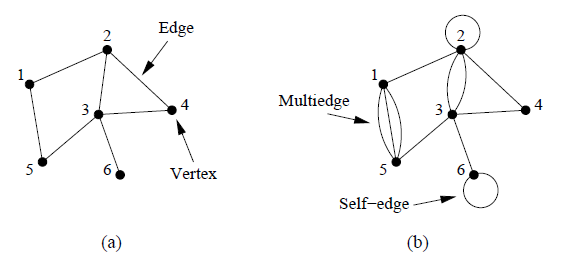
\includegraphics[scale=.8, keepaspectratio]{network_example}
			\caption{(a) Un grafo semplice, cioè privo di self-edge o link multipli. (b) Un grafo che presenta entrambi \cite{Newman}.}
			\label{fig:net_ex}
		\end{center}
	\end{figure}
	
Consideriamo una rete non orientata - cioè una rete in cui i link possono essere percorsi indistintamente in un verso e nell'altro - con $ n $ vertici, che andiamo ad etichettare da $ 1 $ a $ n $. Se indichiamo con $ \left( i, j \right) $ l'arco fra i nodi $ i $ e $ j $, allora l'intera rete può essere descritta in funzione della
\begin{definizione}[\textit{Matrice di adiacenza I}]
La matrice di adiacenza \textbf{A} relativa ad un grafo semplice è una matrice i cui elementi sono così definiti \cite{Newman}:
\[
A_{ij} \, =
\begin{cases}
1, & \text{se esiste un arco fra $ i $ e $ j $};\\ 
0, & \text{altrimenti}.
\end{cases}
\]
\end{definizione}
Se, ad esempio, prendiamo la rete (a) in \cref{fig:net_ex}, assumerà la seguente forma:
\begin{equation}
A =
\begin{pmatrix}
0 & 1 & 0 & 0 & 1 & 0 \\
1 & 0 & 1 & 1 & 0 & 0 \\
0 & 1 & 0 & 1 & 1 & 1 \\
0 & 1 & 1 & 0 & 0 & 0 \\
1 & 0 & 1 & 0 & 0 & 0 \\
0 & 0 & 1 & 0 & 0 & 0
\end{pmatrix} .
\end{equation}
Possiamo osservare che risulta essere una matrice simmetrica con tutti $ 0 $ sulla diagonale. 
\\Qualora invece ne avessimo sotto esame una più simile alla rete (b) della medesima figura, dovremmo tener conto del fatto che sono presenti link multipli e self-edge; si stabilisce di assegnare ai primi un numero pari alla loro molteplicità e ai secondi il valore $ 2 $. Ne risulta una matrice, ancora una volta, simmetrica:
\begin{equation}
A =
\begin{pmatrix}
0 & 1 & 0 & 0 & 3 & 0 \\
1 & 2 & 2 & 1 & 0 & 0 \\
0 & 2 & 0 & 1 & 1 & 1 \\
0 & 1 & 1 & 0 & 0 & 0 \\
3 & 0 & 1 & 0 & 0 & 0 \\
0 & 0 & 1 & 0 & 0 & 2
\end{pmatrix} .
\end{equation}

%\subsection{Digrafi}
%\begin{wrapfigure}{l}{0.4\textwidth}
%		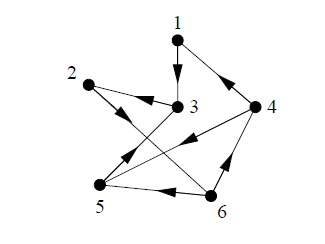
\includegraphics[width=0.38\textwidth]{digraph_example}
%		\caption{Un digrafo \cite{Newman}.}
%		\label{fig:dig_ex}
%\end{wrapfigure}
%La questione cambia leggermente se si va a considerare una rete diretta o \emph{digrafo}.
%\begin{definizione}[\textit{Digrafo}]
%Un \emph{digrafo} è un tipo di grafo in cui ogni arco ha una direzione, punta cioè da un vertice ad un altro \cite{Newman}.
%\end{definizione}
%Ciò ci porta a rivedere quanto detto per la matrice di adiacenza: affermiamo, quindi, che
%\begin{definizione}[\textit{Matrice di adiacenza II}]
%La matrice di adiacenza \textbf{A} relativa ad un grafo orientato è una matrice i cui elementi sono così definiti \cite{Newman}:
%\[
%A_{ij} \, =
%\begin{cases}
%1, & \text{se esiste un arco da $ j $ a $ i $};\\ 
%0, & \text{altrimenti}.
%\end{cases}
%\]
%\end{definizione}
%
%Relativamente alla \cref{fig:dig_ex}, la matrice assumerà, pertanto, la seguente forma: \\
%\begin{equation}
%A =
%\begin{pmatrix}
%0 & 0 & 0 & 1 & 0 & 0 \\
%0 & 0 & 1 & 0 & 0 & 0 \\
%1 & 0 & 0 & 0 & 1 & 0 \\
%0 & 0 & 0 & 0 & 0 & 1 \\
%0 & 0 & 0 & 1 & 0 & 0 \\
%0 & 1 & 0 & 0 & 0 & 0
%\end{pmatrix} .
%\end{equation}
\subsection{Grafi bipartiti}
Ci soffermiamo poi su un ulteriore tipo di grafo, che ci risulterà più utile in seguito.
\begin{definizione}[\textit{Grafo bipartito}] 
Un grafo si dice \emph{bipartito} se i suoi vertici possono essere suddivisi in due sottoinsiemi X e Y tali che ogni link ha un'estremità in X ed una in Y \cite{Bondy}. 
\end{definizione}
\begin{figure}[h]
	\begin{center}
		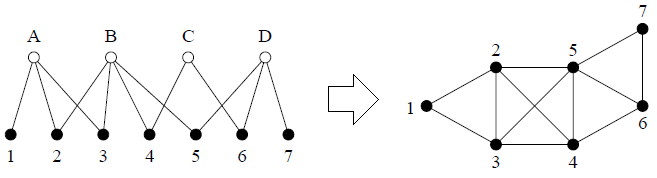
\includegraphics[scale=0.7]{projections2}
		\caption{Passaggio da una rappresentazione tipica di una rete bipartita ad una in cui compaiono solo i vertici \cite{Newman}.}
		\label{fig:proj2}
	\end{center}
\end{figure}

In modo del tutto equivalente a quanto abbiamo già fatto, possiamo andare a definire per un grafo del genere una matrice che lo va a descrivere.
\begin{definizione}[\textit{Matrice di incidenza}]
La matrice di incidenza \textbf{B} è una matrice $ g \times n $, dove $ g $ è il numero di sottoinsiemi e $ n $ quello dei vertici che ne fanno parte, i cui elementi sono definiti come segue \cite{Newman}:
\[
B_{ij} \, =
\begin{cases}
1, & \text{se il vertice $ j $ appartiene al gruppo $ i $ };\\
0, & \text{altrimenti}.
\end{cases}
\]
\end{definizione}

%\begin{wrapfigure}{r}{0.7\textwidth}
%	\begin{center}
%		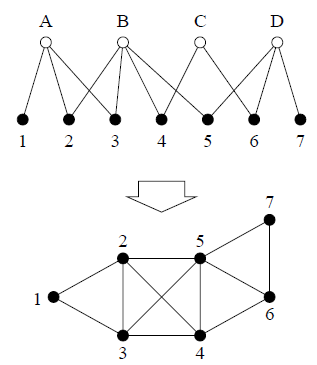
\includegraphics[width=0.35\textwidth]{projections}
%	\end{center}
%	\caption{
%%	In figura si mette in luce il passaggio da una rappresentazione tipica di una rete bipartito ad una in cui compaiono solo i vertici. 
%	\cite{Newman}}
%	\label{fig:projs}
%\end{wrapfigure}
Uno dei pregi di una rete bipartita è quello di consentire in modo fluido il passaggio da una rappresentazione in cui compaiono sia vertici che gruppi ad una in cui, come viene messo in evidenza in \cref{fig:proj2}, sono coinvolti soltanto i vertici; questa possibilità permette di visualizzare il formarsi di quelle che prendono il nome di cricche (\emph{cliques}).
\begin{definizione}[\textit{Cricca}] 
Una \emph{cricca} è un sottografo completo, cioè un sottografo in cui ogni vertice è connesso a tutti gli altri \cite{Bickle}.
\end{definizione}
L'emergere di questi raggruppamenti, di conseguenza, mette in rilievo l'esistenza di gruppi fortemente coesi all'interno della rete; questo aspetto assume ulteriore valore, in particolare, quando cerchiamo di rispondere ad una domanda che ci siamo posti nel precedente capitolo, ovvero come poter rappresentare una popolazione nella quale stia prendendo piede un certo tipo di malattia infettiva, perché ci consente non solo di dare forma agli individui che la costituiscono, ma anche all'intensità dei legami che intercorrono fra di essi: ci aspettiamo, infatti, che membri di una famiglia o colleghi di lavoro vadano a costituire una cricca. 

\section{Grado di un vertice e assortativit\`{a}}
\begin{definizione}[\textit{Grado di un vertice}]
Diciamo \emph{grado} di un vertice il numero di archi ad esso connessi \cite{Lesniak}.
\end{definizione}
Se abbiamo un grafo non orientato con $ n $ vertici, possiamo esprimere il grado dell'i-esimo vertice come
\begin{equation}
	k_i = \sum_{j=1}^n A_{ij}.
\end{equation}
Osserviamo adesso che, se una rete consta di $ m $ link, il numero totale di estremità che possiamo contare - pari a $ 2m $ - altro non è se non la somma dei gradi di tutti i vertici: 
\begin{equation}
	m = \frac{1}{2} \sum_{i=1}^n k_i,
\end{equation}
il che ci porta ad esprimere il grado \emph{medio} di un vertice come 
\begin{equation}
 	c = \frac{1}{2} \sum_{i=1}^n k_i = \frac{2m}{n}. 
\end{equation}
 \\Indichiamo poi la \emph{densità} di un grafo semplice come la frazione di archi effettivamente presenti:
\begin{equation}
	\rho = \frac{m}{\binom{n}{k}} = \frac{2m}{n\left(n-1 \right)} = \frac{c}{n-1}
\end{equation}
con $ 0 \leq \rho \leq  1 $ e  $ \binom{n}{k} $  numero massimo di link che è possibile tracciare. Chiamiamo, infine, \emph{hub} quei nodi che presentano molte connessioni.\\
%Ci soffermiamo brevemente sulle stesse grandezze nel caso in cui si stia esaminando una rete orientata:
%\begin{itemize}
%\item si può distinguere fra il grado esterno (relativo agli archi uscenti da un vertice)
%	\begin{equation}
%		k_{i}^{out} = \sum_{j=1}^n A_{ij}	
%	\end{equation}
%e quello interno (relativo agli archi entranti)
%	\begin{equation}
%		k_{j}^{in} = \sum_{i=1}^n A_{ij}
%	\end{equation}
%\item il numero di link presenti è pari a
%	\begin{equation}
%		m = \sum_{i=1}^n k_i^{in} = \sum_{j=1}^n k_j^{out} = \sum_{ij} A_{ij}
%	\end{equation}
%\item il grado medio esterno è equivalente a quello interno
%	\begin{equation}
%		c^{in} = \frac{1}{n} \sum_{i=1}^n k_i^{in} = \frac{1}{n} \sum_{j=1}^n k_j^{out} = c^{out}.
%	\end{equation}
%\end{itemize}
Il concetto di grado ci è immediatamente utile per definirne un altro: quello di \emph{assortativit\`{a}} o di \emph{mixing assortativo}.
% o meglio scriverli in inglese?
 Con questo termine indichiamo una tendenza, da parte dei vertici, a legarsi con altri nodi che, in qualche modo, somigliano loro; è piuttosto immediato pensare che un aspetto che possono avere in comune sia proprio il grado e, in effetti, in questo contesto si parla di mixing assortativo per grado \cite{Newman}: è possibile andarlo a quantificare mediante un coefficiente di correlazione,
\begin{equation}
	r = \frac{ \sum_{ij} \left( A_{ij} - \frac{k_i k_j}{2m} \right) k_i k_j}{\sum_{ij} \left(k_i \delta_{ij} - \frac{k_i k_j}{2m} \right) k_i k_j} $ . $
\end{equation}

%\medskip
%Per riuscire a rimettere insieme modellazione epidemica e teoria dei grafi, è necessario tener duro ed aggiungere altre definizioni a quelle già introdotte nelle pagine precedenti.
%\begin{definizione}[\textit{Grafo aleatorio}] 
%Per un intero positivo $ n $ e un numero reale $ p $ con $ 0 < p < 1 $, il \emph{grafo aleatorio} $ G \left(n,p \right) $ denota lo spazio delle probabilità i cui elementi sono i $ 2^{\binom{n}{2}} $ diversi grafi che si possono generare a partire da un set di vertici $ \lbrace v_1 \dots v_n \rbrace $ \cite{Lesniak}.
%\end{definizione}
\section{Grafi aleatori}
Una rete reale, tuttavia, non possiede alcun tipo di regolarità, almeno ad un primo sguardo; la difficoltà sta proprio nel riuscire a riprodurre nel miglior modo possibile la disposizione casuale degli archi. A questo proposito andiamo ad introdurre il concetto di \emph{grafo aleatorio}, che viene descritto da una serie di parametri, alcuni dei quali fissati ed altri liberi.
\begin{definizione}[\textit{Modello $ G\left(n,m\right) $}]
Un grafo aleatorio di questo tipo consiste di $ n $ nodi connessi da $ m $ link posizionati casualmente.
\end{definizione}
\begin{definizione}[\textit{Modello $ G\left(n,p\right) $}]
All'interno di questo modello, ciascuna coppia di nodi fra gli $ n $ presenti risulta legata con una probabilità $ p $.
\end{definizione}
Poiché il calcolo di tutta una serie di quantità caratteristiche risulta più semplice nel caso del secondo modello, ci concentreremo essenzialmente su quello \cite{Barabasi}. \\
La probabilità che uno qualunque di tutti i possibili grafi semplici G appaia è
\begin{equation}
P \left(G \right) = p^m \left( 1 - p \right)^{\binom{n}{2} - m}
\end{equation}
ove $ m $ è il numero di archi; pertanto, la probabilità totale di disegnare un grafo con m link a partire dal nostro insieme segue una distribuzione binomiale standard
\begin{equation}
P \left(m \right) = \binom{\binom{n}{2}}{m} p^m \left( 1 - p \right)^{\binom{n}{2} - m}.
\end{equation}
Il numero atteso di archi, di conseguenza, sarà semplicemente:
\begin{equation}
\langle m \rangle = \sum_{m=0}^{\binom{n}{2}} m P \left(m \right) = \binom{n}{2} p,
\end{equation}
mentre il grado medio verrà così calcolato:
\begin{equation}
\langle k \rangle = \sum_{m=0}^{{\binom{n}{2}}} \frac{2m}{n} P \left(m \right) = \left( n - 1 \right) p \doteq c.
\end{equation}

Sulla base di quanto appena detto, quindi, $ p $ è la probabilità che un vertice si leghi con uno qualunque degli altri $ n - 1 $ vertici; ciò ci porta ad esprimere la probabilità totale di essere connesso ad esattamente $ k $ nodi è data da:
\begin{equation}
p_k = \binom{n - 1}{k} p^k \left(1 - p \right)^{n - 1 - k};
\end{equation} 
per $ n \rightarrow \infty $, possiamo andare ad approssimarla come segue

\begin{equation}
p_k  \simeq \frac{ \left(n - 1 \right)^{k}}{k!} p^k e^{- c} = \frac{ \left(n - 1 \right)^{k}}{k!} \left( \frac{c}{ \left(n - 1 \right)} \right)^k e^{- c} = \frac{ c^k e^{- c}}{k!}
\end{equation}
%\begin{split}
%p_k & \simeq \frac{ \left(n - 1 \right)^{k}}{k!} p^k e^{- c} \\
%    & = \frac{ \left(n - 1 \right)^{k}}{k!} \left( \frac{c}{ \left(n - 1 \right)} \right)^k e^{- c} \\
%    & = \frac{ c^k e^{- c}}{k!}
%\end{split}
%\]
cioè $ G \left(n,p \right) $ ha una \emph{distribuzione di grado} poissoniana \cite{Newman}. Distinguiamo due casi limite \cite{Barabasi}:
\begin{itemize}
\item se $ p = 0 $, $ \langle k \rangle = 0 $ e nessun link è presente; \\
\item se $ p = 1 $, $ \langle k \rangle = 1 $ e ogni vertice risulta connesso a tutti gli altri.
\end{itemize} 
Va da sé che, se indichiamo con $ n_g $ la dimensione del più grosso cluster connesso all'interno della rete, nel primo scenario $ n_g = 1 $, mentre nel secondo $ n_g = n $; al crescere di $ \langle k \rangle $ e di conseguenza del rapporto $ \frac{n_g}{n} $, infatti, viene ad emergere quella che indichiamo col nome di \emph{componente gigante} \cite{Erdos}.
\chapter{Percezione del rischio}
\label{chap:cap3}
%Quando parliamo di \emph{modellizzazione ad agenti} intendiamo un tipo di modellizzazione computazionale nel quale un fenomeno viene rappresentato in termine di quelli che vengono chiamati agenti e delle loro interazioni; con \emph{agente} andiamo ad indicare un individuo o un oggetto autonomo in possesso di determinate proprietà e in grado di compiere certe azioni. \\I rapporti fra le varie entità che popolano il modello avvengono localmente, cioè solo fra quelli che vengono considerati \emph{vicini}: è immediato, pertanto, pensare che i soggetti sotto esame si muovano su di una rete e che possano necessariamente avere a che fare solo con chi si trova in loro prossimità. \\ Il primo grande vantaggio derivante dall'uso di questo approccio risiede nel fatto che risulta di più semplice comprensione rispetto ad una rappresentazione di tipo matematico: dal momento che consente di proiettare negli agenti quella che è la nostra esperienza personale, modulata in termini delle interazioni con gli individui coi quali entriamo in contatto, è evidente quanto possa essere più vicino al nostro linguaggio e al nostro modo di pensare. D'altro conto, non si può negare che un'equazione, se risolubile, fornisce in modo diretto un risultato senza il bisogno di far girare un modello, che, specialmente se costituito di un gran numero di agenti, può richiedere un tempo di esecuzione talmente lungo da renderlo poco funzionale \cite{Rand}. Un ulteriore merito del quale è necessario prendere atto è la sua capacità di mettere in luce il fenomeno dell'\emph{emergenza}, cioè di tutto quell'insieme di comportamenti e proprietà che vengono fuori dall'interazione di singoli individui e che non risultano predicibili a partire dalle caratteristiche di questi ultimi; ciò è possibile perché si tratta di un approccio "across-levels", secondo il quale gli agenti non vengono considerati avulsi dall'ambiente in cui sono immersi, ma viene dato particolare rilievo alla reciproca influenza fra i due. \\ Non sarà sorprendente, a questo punto, affermare che il processo di modellizzazione sottostà ad una serie di passi che possono venire iterati più volte - dando luogo a quello che chiamiamo "modeling cycle" - in modo da rendere il modello il più efficace ed efficiente possibile:
%\begin{enumerate}
%\item \textit{formulazione delle domande}, per meglio mettere a fuoco il problema che si vuole analizzare;
%\item \textit{costruzione delle ipotesi}, che devono inizialmente essere il più semplici possibili, per venir poi rinforzate ed arricchite più avanti nel processo;
%\item \textit{scelta delle variabili di stato e dei parametri}, per iniziare a mettere per iscritto il modo in cui ci aspettiamo che il nostro modello si comporti;
%\item \textit{implementazione del modello}, che consente di esplorare e valutare se le assunzioni fatte sono valide ed hanno prodotto un che di utile;
%\item \textit{analisi, test e revisione}, così da apportare modifiche o migliorie;
%\item \textit{comunicazione del modello} \cite{Grimm}.
%\end{enumerate}
%In ultimo, è interessante sottolineare, seppur brevemente, quale sia il ruolo epistemico della simulazione computazionale: è, infatti, possibile attribuirle un potere sia \emph{esplicativo}, poiché permette di comprendere come si siano verificati alcuni eventi, sia \emph{predittivo}, dal momento che rende possibile immaginare il comportamento futuro di un sistema sotto determinate circostanze, che \emph{esplorativo}, in quanto fa sì che le informazioni che intendiamo rappresentare possano essere condivise e rese note ad altri \cite{Primiero}.
%\\ All'interno di questo lavoro di tesi faremo uso di Netlogo, che è sia un IDE, ovvero un ambiente di sviluppo integrato, che un linguaggio di modellazione; è stato progettato nel $ 1999 $ col fine di rendere il più semplice possibile la costruzione di modelli basati su agenti. Nella fattispecie, utilizzeremo la versione $ 6.2.0 $; per ulteriori dettagli tecnici, rimandiamo alla documentazione ufficiale \cite{Wilensky}.
Un elemento sul quale vorremo concentrare la nostra attenzione è la \emph{percezione del rischio}, poiché ci aspettiamo che possa rappresentare un fattore chiave nell'andamento dell'epidemia. Si osserva, infatti, che, qualora ci si trovi di fronte ad una malattia i cui sintomi sono evidentemente manifesti, le persone modificano il proprio comportamento e le proprie abitudini sulla base della propria soggettiva sensazione di pericolo; ad esempio, potrebbero prediligere l'uso di un mezzo di trasporto privato, rispetto ad uno pubblico, per recarsi a lavoro, in modo da limitare le occasioni di contatto con estranei. È altresì vero che la percezione del rischio varia anche col grado di intimità che si ha con un determinato individuo: in linea di massima, la tendenza è quella di temere meno l'infezione se ci si trova in compagnia di un familiare o di un amico, mentre in presenza di estranei il livello di allerta si fa ben più alto. \\Per amore di semplicità, in questo lavoro assumeremo che tutti i soggetti percepiscano il rischio e reagiscano ad esso allo stesso modo: facciamo, cioè, un'ipotesi di \emph{popolazione omogenea}. Aggiungiamo due ulteriori supposizioni:
\begin{enumerate}
	\item la malattia si rende visibile nel medesimo momento in cui infetta qualcuno;
	\item la percezione del rischio è proporzionale alla frazione di contatti con individui infetti rispetto alla totalità dei contatti \cite{Bagnoli2007}.
\end{enumerate}
\section{Il modello e l'approssimazione di campo medio}
Poniamo la nostra attenzione su reti costituite da $ N $ nodi e $ 2mN $ link. Come già fatto in precedenza, andiamo ad indicare con $ a_{ij} $ l'ij-esimo elemento della matrice di adiacenza - pari a 1 se esiste un arco da j a i e $ 0 $ altrimenti - e con $ k_i = \sum_{j} a_{ij} $ la connettività del sito $ i $ - così che risulta $ \langle k \rangle = 2m $ - ; denotiamo, invece, quella dei suoi vicini come $ j_{1}^i \dots j_{k_{i}}^i $. Andiamo a sostituire alla probabilità d'infezione netta, indicata con la lettera $ \tau $, la quantità $ u\left(s,k \right) $: nello specifico, questa può esplicitamente essere scritta come
\begin{equation}
	u\left(s,k_i \right) = \tau \exp(-J \tfrac{s}{k_i})
	\label{infect_sk}
\end{equation}
e va a rappresentare la probabilità che il sito $ i $, avente connettività $ k_i $, contragga l'infezione da uno degli $ s $ vicini malati \cite{Bagnoli2014}. Quanto appena scritto riflette in pieno quanto asserivamo poco sopra, ovvero che l'eventualità di venire contagiati diminuisca in funzione della percezione del rischio, data dalla percentuale di vicini infetti e modulata da un fattore $ J $, che può dipendere dal tipo di misure di precauzione adottate. 
%\section{Approssimazione di campo medio}
\\La più semplice approssimazione di campo medio che è possibile formulare richiede di trascurare l'eventuale correlazione fra le variabili; in altre parole, si assume che non ci siano loop. 
\subsection{Generazione di una rete poissoniana}
Poniamoci nel caso in cui la rete che rappresenta i contatti sia aleatoria: ciò significa che ciascun nodo forma un numero $ m $ di link con altrettanti vertici scelti in modo casuale e che la distribuzione di grado segue una poissoniana. Inoltre, stabiliamo che $ k $ sia fissato: allora, se indichiamo con $ c $ la frazione di infetti al tempo $ t $ e con $ c' $ quella al tempo immediatamente successivo $ t + 1 $, possiamo scrivere che
\begin{equation}
c' = \sum_{s = 0}^k \binom{k}{s}c^s \left(1-c \right)^{k-s} p\left(s,k \right),
\end{equation}
laddove $ p\left(s,k \right) = 1 - \left[1 - u \left(s,k \right) \right]^s$ è la probabilità di ammalarsi se sono presenti $ s $ vicini infetti su $ k $ \cite{Bagnoli2014}. 
\medskip
\\Apriamo, a questo punto, una doverosa parentesi ed introduciamo un ulteriore concetto caro alla teoria dei grafi: la \emph{percolazione}, ovvero la rimozione di un vertice di una rete (p. \emph{di sito}) oppure quella di un arco (p. \emph{di legame}). In questo contesto, possiamo affermare che un link viene occupato con una probabilità $ \phi $; link di questo tipo sono quelli lungo cui può essere trasmessa l'infezione. Al crescere di  $ \phi $, nodi inizialmente isolati si fanno via via più grandi, fino ad arrivare a creare un cluster unico  che altro non è se non quella che abbiamo chiamato componente gigante e che raggiunge la sua dimensione massima per $ \phi = 1 $; questo fenomeno prende il nome di \emph{transizione di percolazione}. Quello che si può arrivare a dire è che la soglia di percolazione su di una rete coincide con la soglia epidemica per la diffusione di una malattia sulla medesima rete: infatti, per valori piccoli di $ \phi $ il primo infetto appartiene necessariamente ad un cluster di dimensioni modeste e, di conseguenza, la maggior parte della popolazione non viene infettata; al contrario, quando $ \phi $ è grande, aumenta il numero di vertici facenti parte della componente gigante e, di pari passo, la probabilità che il paziente zero vi faccia parte e dia l'avvio ad una vera e propria ondata epidemica \cite{Newman}.
\medskip
\\Torniamo al nostro problema. Ci aspettiamo che in prossimità della soglia di percolazione/epidemica la \eqref{infect_sk} sia piccola, il che ci consente di approssimare
\begin{equation}
	c' \simeq \sum_{s = 0}^k \binom{k}{s}c^s \left(1-c \right)^{k-s} s \, \tau \, exp(-J \tfrac{s}{k});
\end{equation}
ponendo $ a \doteq exp(- \tfrac{J}{k}) $, si trova che
\begin{equation}
	c' = \tau a k \left(c a + 1 - c \right)^{k-1}.
\end{equation}
La soglia critica $ J_c $ corrisponde allo stato stazionario $ c = c' $, nel limite $ c \rightarrow 0 $:
\begin{equation}
	\tau = \frac{1}{k} exp(\tfrac{J_c}{k}),\quad J_c = k \ln(k \tau).
\end{equation}

\begin{figure}[t]
		\begin{center}
			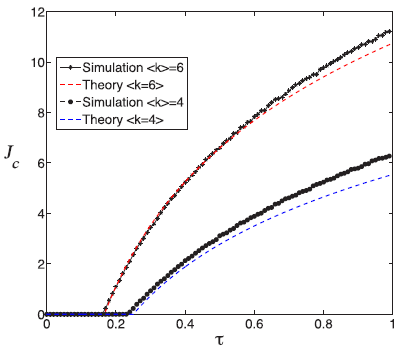
\includegraphics[scale=.8, keepaspectratio]{mean_field_sim}
			\caption{Confronto fra l'approssimazione di campo medio e le simulazioni condotte per una rete aleatoria al variare di $ \langle k \rangle $ \cite{Bagnoli2014} .}
			\label{fig:sim}
		\end{center}
\end{figure}
La nostra predizione è piuttosto precisa: ce lo confermano le simulazioni eseguite, come possiamo osservare in \cref{fig:sim}.

\subsection{Generazione di una rete scale-free}
Vediamo adesso cosa cambia se prendiamo in esame una rete a invarianza di scala o \emph{scale-free}: reti siffatte sono descritte da una distribuzione di grado data da $ P\left(k\right) = A k^{-\alpha} $, con $ A $ costante e, in genere, $ 2 \leq \alpha \leq 3 $ \footnote{In realtà, la distribuzione di grado di una rete scale-free non segue pedissequamente l'andamento di una legge di potenza: questa ultima, infatti, risulta essere sempre una funzione monotona decrescente su tutto il proprio dominio, mentre capita che $ P\left(k\right) $ si comporti come atteso solo in prossimità delle code della distribuzione.}. 
%aggiungere nota a piè di pagina per precisazione su reti scale-free?
Imponiamo che il grado di ciascun nodo sia limitato, $ m \leq k \leq K $ \footnote{Può succedere che $ P\left(k\right)$ devii anche in corrispondenza di $ k $ grande; si introduce perciò un taglio $ K $ di qualche tipo in modo da andare a limitare il grado massimo dei vertici \cite{Newman}.}; 
%nota a piè di pagina per il taglio K
consci del fatto che $ \sum_{k = 0}^K p_k = 1 $, possiamo normalizzare e ricavare il valore di $ A $, cioè $ A = \tfrac{ \alpha - 1}{m^{1 - \alpha} - K^{1 - \alpha}} $. \\ Utilizzando lo stesso formalismo impiegato in precedenza, possiamo prima di tutto esprimere lo stato di un nodo con connettività $ k $ al tempo $ t + 1 $ nel modo seguente:
\begin{equation}
	c'_k = \sum_{s_1 \dots s_k = 0}^1 \, \sum_{j_1 \dots j_k = 0}^ \infty \, \prod_{i = 1}^k C\left(j_i,k\right) I\left(s_i, j_i\right) T\left(k|s_i\right),
\end{equation}
dove l'indice $ i = 1, \dots, k $ corre sul numero dei vicini e $ s_i = 0, 1 $ esprime il loro stato (rispettivamente, sani e infetti). $ C\left(j,k)\right) $ è la probabilità che un nodo con connettività $ j $ sia legato ad un altro con connettività $ k $, $ I\left(s_i, j_i\right) $ quella che l'$ i $-esimo vicino sia malato e $ T\left(k|s_i\right) $, infine, quella che possa trasmettere l'infezione al nodo sotto esame. \\ Osservando che è possibile riscrivere
\begin{itemize}
	\item $ C\left(j,k)\right) = \frac{j P\left(j\right)}{\langle k \rangle} $ (in quanto per reti simmetriche vale $ j C\left(j,k\right) P\left(j\right) = k C\left(k,j\right) P\left(k\right) $),
	\item $ I\left(s_i, j_i\right) = c_{j_i}^{s_i} \left(1 - c_{j_i}\right)^{1 - s_i} $,
	\item $ T\left(k|s_i\right) = 1 - \left(1 - \tau \, exp(- \tfrac{J s}{k})\right)^s \simeq s \, \tau \, exp(- \tfrac{J s}{k}) $
\end{itemize}
e definendo $ \tilde{c} \doteq \sum_j j \tfrac{P\left(j\right) c_j}{\langle k \rangle} $, possiamo concludere che \cite{Bagnoli2014}
\begin{equation}
	c'_k = \tilde{c} \, k \, \tau \quad exp(- \tfrac{J s}{k}) \left(\tilde{c} \, exp(- \tfrac{J}{k}) + 1 - \tilde{c}\right).
\end{equation}
In prossimità della soglia epidemica, $ \tilde{c} \to 0 $; questo ci permette di ricavare nuovamente la relazione fra $ \tau_c $ e $ J_c $:
\begin{equation}
	\tau_c\left(J_c\right) = \frac{\langle k \rangle}{\sum_k k^2 P\left(j\right) \, exp(-\tfrac{J_c}{k})}.
\end{equation}
L'espressione soprastante può essere esplicitata se ci si pone nel limite continuo e si mettono in atto le opportune sostituzioni; infatti, per $ K \gg m $, si ottiene che
\begin{equation}
	\tau_c \left(J_c \right) = J_{c}^{3 - \alpha} \left[ \Gamma \left( \alpha - 3, \tfrac{J_c}{k} \right) - \Gamma \left( \alpha - 3, \tfrac{J_c}{m}\right) \right] 	 
\end{equation}
%\footnote{$ \Gamma \left(a,x\right)$ è la funzione gamma incompleta}
che risulta evidentemente divergente per $ K \to \infty $ - il che ci fa concludere che $ J_c = 0 \, \forall \tau$ -. Una rete reale, d'altra parte, possiede sempre un numero finito di nodi, per cui anche il taglio deve essere tale; questo ci consente di valutare $ \tau $ per $ J_c = 0 $:
\begin{equation}
	\tau_c\left(0\right) = \frac{\alpha - 3}{\alpha - 2} \frac{m^{2 - \alpha} - K^{2 - \alpha}}{m^{3 - \alpha} - K^{3 - \alpha}} \simeq \frac{3 - \alpha}{\alpha - 2} \frac{m^{2 - \alpha}}{K^{3 - \alpha}}
	\label{tau_zero}
\end{equation}

\begin{figure}[t]
		\begin{center}
			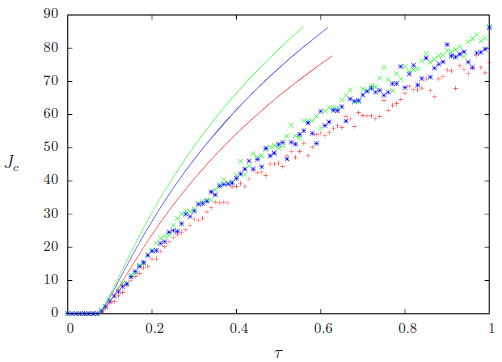
\includegraphics[scale=.8, keepaspectratio]{mean_field_sim2}
			\caption{Confronto fra l'approssimazione di campo medio (le curve) e le simulazioni condotte per $ 3 $ diversi casi di reti scale-free con $ \alpha = 2.4, \, N = 10000, \, m = 2, \, K = 300 $ \cite{Bagnoli2014} .}
			\label{fig:sim2}
		\end{center}
\end{figure}
Notiamo in \cref{fig:sim2} che, stavolta, c'è un buon accordo fra il modello teorico e i risultati ottenuti dalle simulazioni solo per $ J_c = 0 $; oltrettutto, il valore di $ \tau_c\left(0\right) $ ottenuto a partire dall'approssimazione continua \eqref{tau_zero}, $ \tau\left(0\right) \simeq 0.037 $, è piuttosto diverso da quello calcolato mediante le simulazioni, $ \tau\left(0\right) \simeq 0.08 $. 
\section{Risultati}
Quello che possiamo affermare è che, a prescindere dal tipo di rete che andiamo a generare, l'adozione di un livello di precauzione $ J $ sufficientemente alto da parte di tutti gli agenti consente di fermare la diffusione epidemica anche se si è oltrepassata la soglia $ \tau_c $ \cite{Bagnoli2014}.

% \addcontentsline{toc}{chapter}{Conclusioni}
% \chapter*{Conclusioni}
\chapter{Simulazioni con la modellizzazione ad agenti}
\label{chap:cap4}
Come già accennato nel primo capitolo, in questo lavoro di tesi ci siamo serviti di NetLogo al fine di costruire un modello di diffusione epidemica su rete; in particolare, abbiamo fatto uso di BehaviorSpace, uno strumento software, messo a disposizione da NetLogo stesso, che consente di eseguire più volte un esperimento andandone a variare alcuni parametri caratteristici \cite{Wilensky2}. 
\section{Il modello}
Il nostro obiettivo è quello di andare a valutare come varia la frazione di individui che non contraggono mai l'infezione al mutare della percezione del rischio; al suo aumentare ci aspettiamo, abbastanza intuitivamente, che il processo diffusivo si arresti prima e che, quindi, il numero di soggetti che non si sono ammalati diventi via via maggiore. \\Il modello compartimentale preso in considerazione è il SIS (Suscettibili - Infetti - Suscettibili), che non prevede l'acquisizione di alcun tipo di immunità una volta guariti dall'infezione \cite{Brauer}. 
La diffusione dell'epidemia avviene su una rete generata algoritmicamente attraverso la procedura \texttt{to-create-network} \footnote{Si consulti l'appendice per il codice completo e commentato.}; il numero di nodi che la costituiva poteva variare da un minimo di $ 2 $ ad un massimo di $ 1000 $, ma si è scelto di mantenere l'indicatore su di questo ultimo valore per tutte le simulazioni condotte.
%Affinché fosse più immediato visualizzarne l'evoluzione nel tempo, abbiamo generato una rete con un numero di nodi ("num-nodes") che poteva variare da un minimo di $ 2 $ ad un massimo di $ 1000 $; si è scelto di mantenere l'indicatore su di questo ultimo valore per tutte le simulazioni condotte.
 \`{E} stato anche possibile controllare mediante slider (\texttt{preferential-attachment}) la probabilità che un nuovo nodo risultasse legato ad un altro già altamente connesso: ciò ha consentito di dare origine sia a reti totalmente aleatorie che a reti di tipo scale-free. \\Altri parametri presi in considerazione - anch'essi modificabili tramite un cursore - sono stati:
\begin{itemize}
\item \textit{la frazione iniziale di infetti} (\texttt{fraction-infected});
\item \textit{il tasso di infettività} (\texttt{infectivity});
\item \textit{il livello di misure di precauzione} individuali, indicato genericamente come \texttt{risk-perception}, ma coincidente con la quantità $ J $ definita nel precedente capitolo.
\end{itemize}
\begin{figure}[t]
		\begin{center}
			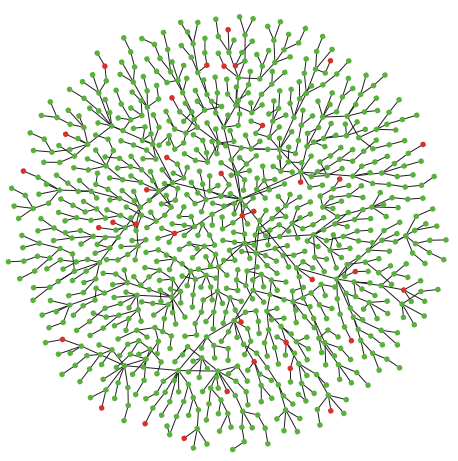
\includegraphics[scale=.65, keepaspectratio]{network_w_Netlogo_2}
			\caption{Esempio di rete generata dal nostro codice dopo aver impostato \texttt{num-nodes} $= 1000 $, \texttt{preferential-attachment} $= 0.00 $ e \texttt{infected-fraction} $= 0.031 $.}
			\label{fig:NetLogo1}
		\end{center}
\end{figure}
%Ricordiamo, a questo proposito, di aver sostituito alla probabilità di infezione netta $ \tau $ il prodotto $ \tau \cdot exp(-J \tfrac{s}{k}) $, dove con $ \tfrac{s}{k} $ si è indicato la frazione $ s $ di infetti su $ k $ vicini; nel codice sviluppato questa quantità è stata resa dalla variabile "alert" 
Gli agenti - che su NetLogo vengono indicati con il nome di \texttt{turtles} - possono essere descritti in termini di tre variabili:
\begin{enumerate}
\item \texttt{state}, alla quale viene assegnato un valore numerico $ \geq 0 $ sulla base della condizione di salute e che, pertanto, funge da contatore per la durata del periodo d'infezione;
\item \texttt{infected?}, che può assumere valore booleano;
\item \texttt{alert}, che tiene conto della quantità di vicini infetti e che, nel precedente capitolo, veniva quantificata dal rapporto $ \tfrac{s}{k}$.
\end{enumerate}
Come viene reso evidente in \cref{fig:NetLogo1}, i nodi di colore rosso sono quelli infetti; il loro numero viene stabilito a seguito dell'estrazione di un numero casuale fra $ 0 $ e $ 1 $ e del confronto di questo con la quantità \texttt{initial-infected}. La probabilità che contagino i vertici ai quali sono collegati è anch'essa aleatoria:
\begin{center}
	\begin{lstlisting}[autogobble,language={NetLogo},caption={Porzione di codice in cui si implementa il meccanismo di infezione.},label={list:infection_prob}]
		ask turtles with [state > 0] [
    		ask out-link-neighbors with [state = 0] [
      			if random-float 1 < infectivity * exp(-1 * risk-perception * alert) [
        				set state num-states
        				set infected? true
      			]
    		]
  		]  
	\end{lstlisting}
\end{center}
%\begin{center}
%\begin{lstlisting}[language={NetLogo},caption={Porzione di codice in cui si mette in luce il meccanismo di infezione.},label={list:infection_prob}]
%		ask turtles with [state > 0] 
%    		ask out-link-neighbors with [state = 0] 
%      			if random-float 1 < infectivity * exp(-1 * risk-perception * alert) 
%        				set state num-states
%        				set infected? true]]]
%\end{lstlisting}
%\end{center}
Si rimanda all'appendice \ref{appendix:code} per il codice sviluppato per intero.
\section{Analisi sperimentale}
Abbiamo deciso di eseguire una serie di simulazioni sia per una rete poissoniana che per una scale-free. In entrambe le casistiche, abbiamo mantenuto fissati tutti i parametri in gioco meno \texttt{perception-risk}, che, invece, abbiamo fatto variare da $ 0.10 $ a $ 0.35 $ a passi di $ 0.05 $; abbiamo poi stabilito di ripetere ogni operazione $ 10 $ volte. I valori comuni che abbiamo impostato sono i seguenti:
\begin{itemize}
\item numero di nodi (\texttt{num-nodes}) $ = 1000 $;
\item tasso di infettività (\texttt{infectivity}) $ = 0.2 $;
\item numero iniziale di infetti (\texttt{initial-infected}) $ = 0.031 $;
\item durata dell'infezione (\texttt{num-states}) $ = 4 $.
\end{itemize}
%\subsection{Caso I: rete poissoniana}
%Abbiamo messo lo slider "preferential-attachment" a $ 0.00 $ ed abbiamo avviato BehaviorSpace; abbiamo atteso che portasse a compimento tutte le esecuzioni
%
%\subsection{Caso II: rete scale-free}
%Per questo scenario, abbiamo impostato lo slider "preferential-attachment" su $ 0.60 $.
L'unica differenza, per quanto riguarda gli slider gestibili dall'utente, sta nel fatto che nel primo caso abbiamo messo \texttt{preferential-attachment} pari a $ 0.00 $  - così che la rete generata fosse totalmente aleatoria - mentre nel secondo l'abbiamo posto pari a $ 0.60 $ (si noti la diversa disposizione dei link in \cref{fig:NetLogo2}).
\begin{figure}[t]
		\begin{center}
			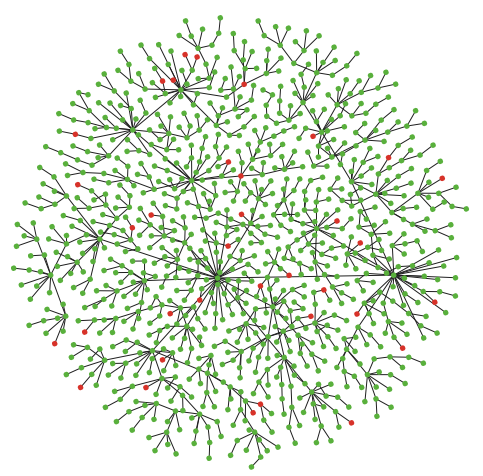
\includegraphics[scale=.65, keepaspectratio]{network_w_Netlogo_3b}
			\caption{Esempio di rete generata dopo aver impostato \texttt{num-nodes} $= 1000 $, \texttt{preferential-attachment} $= 0.60 $ e \texttt{infected-fraction} $= 0.031 $.}
			\label{fig:NetLogo2}
		\end{center}
\end{figure}
\\Ad ogni lancio del programma, viene decrementata di un'unità la variabile \texttt{state}, che, per un individuo infetto, ha valore iniziale pari a \texttt{num-states}; quando \texttt{state} torna uguale a $ 0 $, si assume che il soggetto sia guarito e il nodo che lo va a rappresentare passa dal rosso al giallo \footnote{Nonostante tornino a fare parte del gruppo dei suscettibili (dal momento che stiamo considerando un modello SIS), preferiamo non colorare di verde gli agenti che si sono ristabiliti dalla malattia per poterli distinguere da quelli che non l'hanno mai contratta.}. Inoltre, ogni agente suscettibile conta il numero di vicini - cioè di nodi che ad esso sono collegati - infetti e imposta questo valore come \texttt{alert}; viene poi messo in atto il processo di infezione come mostrato nella porzione di codice \ref{list:infection_prob}. \\Poiché siamo interessati, come già sottolineato, alla frazione di soggetti che non si sono mai ammalati, ne prendiamo nota con la procedura 
\begin{center}
	\begin{lstlisting}[autogobble,language={NetLogo},caption={Metodo che riporta la frazione di suscettibili che non hanno mai contratto l'infezione.},label={list:count_susceptibles}]
		to-report fraction-susceptibles
  			report count turtles with [infected? = false] / count turtles
		end	
	\end{lstlisting}
\end{center}
che viene successivamente sfruttata da BehaviorSpace per stampare il dato ricercato su di un file CSV. \\ Questa operazione viene ripetuta ad ogni \texttt{tick}, cioè ad ogni istante di tempo. Per evitare che la nostra simulazione avesse una durata di esecuzione infinita, abbiamo aggiunto due stop ad hoc: il primo nel caso in cui si riesca ad estirpare l'epidemia e quindi non ci siano più agenti infetti, il secondo qualora le precauzioni prese non siano sufficienti e la malattia raggiunga tutti gli individui facenti parte della rete.
\section{Risultati e considerazioni finali}
Riportiamo di seguito i risultati delle nostre simulazioni.
%\begin{figure*}
%	\begin{minipage}{0.48\textwidth}
%		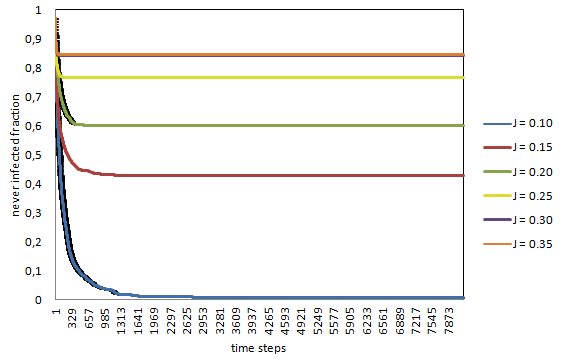
\includegraphics[scale = 0.3]{poisson_errorbars_I}
%		\caption{Andamento della frazione dei suscettibili, nel caso di una rete poissoniana, in funzione di una diversa percezione del rischio.}
%	\end{minipage}
%\hfill
%	\begin{minipage}{0.48\textwidth}
%		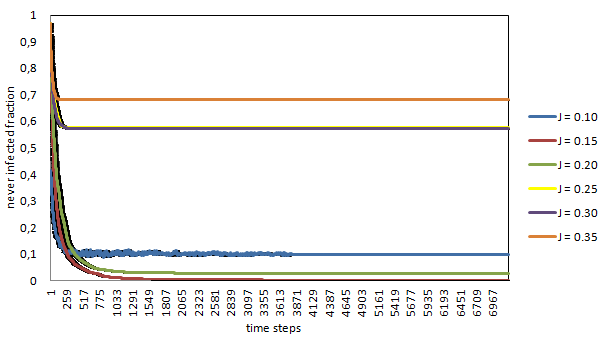
\includegraphics[scale = 0.3]{scalefree_errorbars_I}
%	\caption{Andamento della frazione dei suscettibili, nel caso di una rete scale-free, in funzione di una diversa percezione del rischio.}
%	\end{minipage}
%\end{figure*}
%\begin{figure}
%		\begin{center}
%			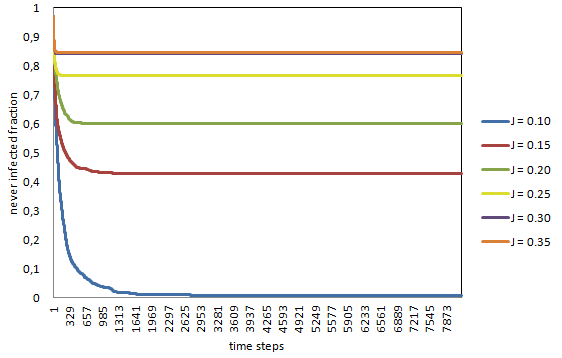
\includegraphics[scale=.7, keepaspectratio]{poisson_I}
%			\caption{Andamento della frazione dei suscettibili, nel caso di una rete poissoniana, in funzione di una diversa percezione del rischio.}
%			\label{fig:sim_poisson}
%		\end{center}
%\end{figure}
%
%\begin{figure}
%		\begin{center}
%			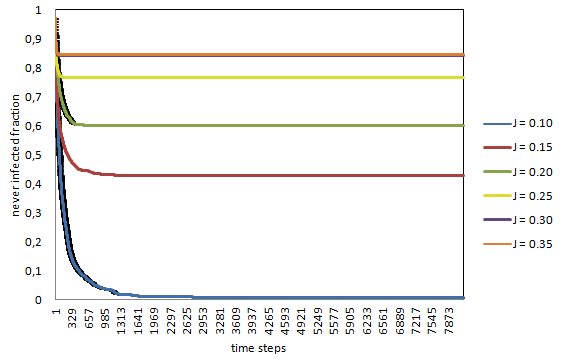
\includegraphics[scale=.7, keepaspectratio]{poisson_errorbars_I}
%			\caption{Come in \cref{fig:sim_poisson} ma con barre d'errore.}
%			\label{fig:sim_poisson2}
%		\end{center}
%\end{figure}
%
%\begin{figure}
%		\begin{center}
%			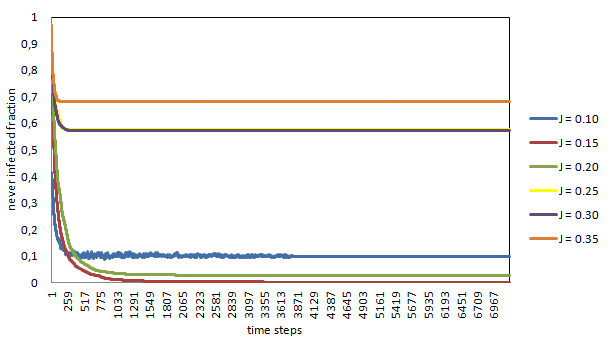
\includegraphics[scale=.7, keepaspectratio]{scalefree_I}
%			\caption{Andamento della frazione dei suscettibili, nel caso di una rete scale-free, in funzione di una diversa percezione del rischio.}
%			\label{fig:sim_scalefree}
%		\end{center}
%\end{figure}	
%
%\begin{figure}
%		\begin{center}
%			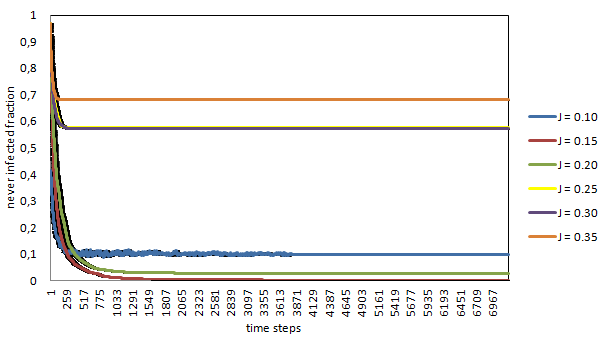
\includegraphics[scale=.7, keepaspectratio]{scalefree_errorbars_I}
%			\caption{Come in \cref{fig:sim_scalefree} ma con barre d'errore.}
%			\label{fig:sim_scalefree2}
%		\end{center}
%\end{figure}	
\begin{figure}
		\begin{center}
			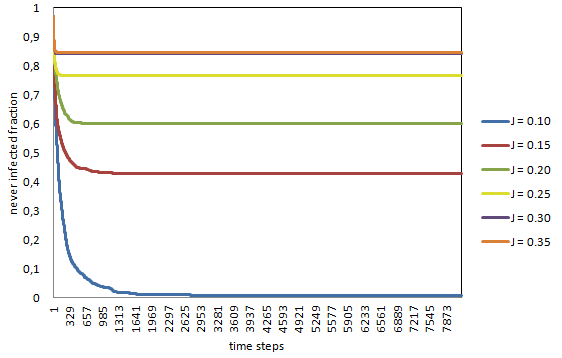
\includegraphics[width=0.85\textwidth]{poisson_I}
			\caption{Andamento della frazione dei suscettibili, nel caso di una rete poissoniana, in funzione di una diversa percezione del rischio.}
			\label{fig:sim_poisson}
		\end{center}
\end{figure}
%
\begin{figure}
		\begin{center}
			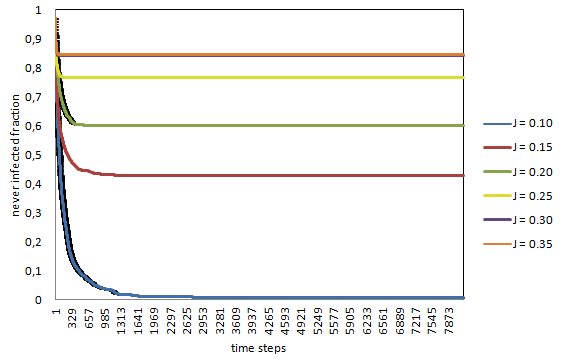
\includegraphics[width=0.85\textwidth]{poisson_errorbars_I}
			\caption{Come in \cref{fig:sim_poisson} ma con barre d'errore.}
			\label{fig:sim_poisson2}
		\end{center}
\end{figure}
%
\begin{figure}
		\begin{center}
			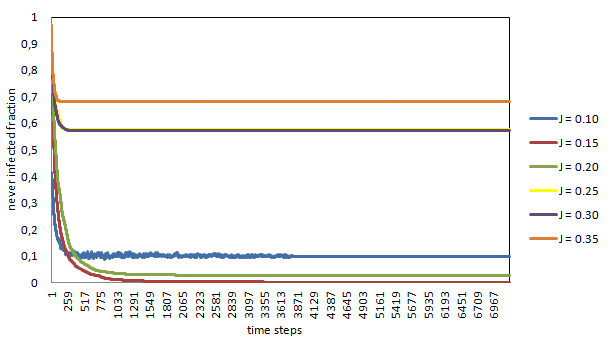
\includegraphics[width=0.85\textwidth]{scalefree_I}
			\caption{Andamento della frazione dei suscettibili, nel caso di una rete scale-free, in funzione di una diversa percezione del rischio.}
			\label{fig:sim_scalefree}
		\end{center}
\end{figure}	
%
\begin{figure}
		\begin{center}
			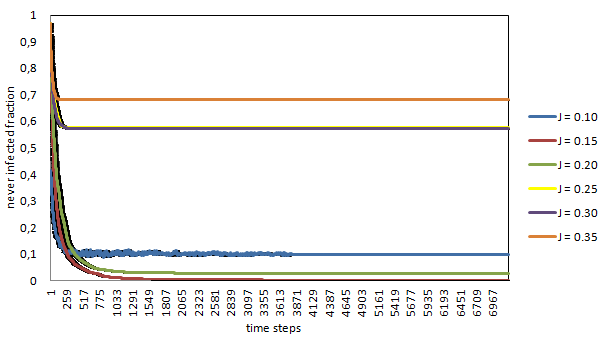
\includegraphics[width=0.85\textwidth]{scalefree_errorbars_I}
			\caption{Come in \cref{fig:sim_scalefree} ma con barre d'errore.}
			\label{fig:sim_scalefree2}
		\end{center}
\end{figure}	
\\Nel caso di una rete aleatoria, quello che è emerso è che basta cambiare anche di poco il valore di $ J $ per ottenere frazioni significativamente diverse degli agenti rimasti sani per tutta la durata delle simulazioni (basti confrontare l'andamento per $ J = 0.10 $ e per $ J = 0.15 $); in aggiunta, si noti in \cref{fig:sim_poisson} che per $ J \geq 0.30 $ le curve ottenute si fanno praticamente indistinguibili, il che potrebbe far ipotizzare che esista un valore di soglia per $ J $ oltre il quale non si registrano grosse differenze nel numero di individui che non hanno contratto l'infezione \footnote{Per andare a verificare questa supposizione, dovremmo ripetere l'intero esperimento facendo variare $ J $ in un range più ampio.}. \\Come ci aspettavamo, non avviene lo stesso nel caso scale free; difatti, se si tiene sott'occhio la \cref{fig:sim_scalefree}, si può osservare che non si verificano miglioramenti apprezzabili se non a partire da $ J = 0.25 $. Questo comportamento è strettamente legato alla struttura della rete: la presenza di \emph{hub}, cioè di nodi molto connessi, ha reso più complicata l'estinzione dell'epidemia proprio perché questi, in potenza, contagiano un numero di vicini ben più grande rispetto ad un vertice più isolato. Del resto, sarebbe sufficiente osservare anche solo una singola simulazione del modello NetLogo per convincersene: quand'anche la percezione del rischio fosse relativamente alta, se un hub contrae l'infezione è altamente probabile che tutti i nodi che gli sono collegati facciano la stessa fine, mentre è piuttosto verosimile che agenti nella periferia della rete non entrino mai in contatto con la malattia. Si conferma, perciò, uno dei risultati messi in evidenza in \cite{Bagnoli2007}, ovvero la necessità che gli individui con un elevato numero di contatti adottino misure di precauzione più stringenti rispetto al resto della popolazione al fine di porre un ulteriore freno al diffondersi dell'infezione.
% \addcontentsline{toc}{chapter}{Conclusioni}
% \chapter*{Conclusioni}
\chapter{Conclusioni}
\label{chap:conclusioni}
Al giorno d'oggi, quello della modellazione epidemica è un processo che assume un'importanza sempre più centrale: un motivo fra tanti risiede nel fatto che, una volta che se ne sono appresi i meccanismi di trasmissione, rende possibile l'elaborazione di una serie di strategie volte ad ostacolarla. A questo proposito, è utile andare a suddividere la popolazione in compartimenti, ciascuno descrittivo dello stato di salute degli individui che ne fanno parte; così facendo, il nostro problema può essere interpretato in chiave della probabilità di transizione fra un gruppo e l'altro. La nostra rappresentazione si arricchisce di un ulteriore tassello nel momento in cui si descrivono i contatti fra soggetti come gli archi di una rete i cui nodi sono le persone stesse. 
\medskip
\\
%In questo lavoro di tesi ci siamo concentrati sull'influenza che la percezione del rischio ha nella diffusione di una malattia infettiva; per far ciò, ci siamo basati sulle assunzioni abbiamo assunto che la probabilità di venire contagiati fosse modulata da altri due fattori, la frazione di contatti infetti e l'insieme di misure precauzionali assunte, che, complessivamente, hanno come effetto quello di diminuirla. Siamo partiti da un modello epidemico sviluppato su rete e, grazie all'utilizzo di BehaviorSpace, siamo riusciti a effettuare un certo numero di simulazioni: questo ci ha permesso di ripetere più volte l'esperimento e di indagare i diversi scenari di trasmissione che si sono originati dalle medesime condizioni iniziali. 
In questo lavoro di tesi ci siamo concentrati sull'influenza che la percezione del rischio ha nella diffusione di una malattia infettiva. Per far ciò ci siamo basati su un modello epidemico sviluppato su rete da Bagnoli \textit{et al.} in \cite{Bagnoli2014} e \cite{Bagnoli2007}; in particolar modo, abbiamo sfruttato l'assunto secondo cui la probabilità di venire contagiati venga modulata da altri due fattori, la frazione di contatti infetti e l'insieme di misure precauzionali assunte (rappresentato dal parametro $ J $), che, complessivamente, hanno come effetto quello di diminuirla. Abbiamo importato tale modello in un contesto ad agenti, al fine di simulare, a partire dalle medesime condizioni iniziali, diversi scenari di trasmissione e di indagare come la differente percezione del rischio vada ad impattare sul numero di soggetti che non sono mai stati esposti al contagio. 
\medskip
\\
%
%\\Nel caso di una rete aleatoria, quello che è emerso è che basta cambiare anche di poco il valore di $ J $ per ottenere frazioni significativamente diverse degli agenti rimasti sani per tutta la durata delle simulazioni (basti confrontare l'andamento per $ J = 0.10 $ e per $ J = 0.15 $); in aggiunta, si noti in \cref{fig:sim_poisson} che per $ J \geq 0.30 $ le curve ottenute si fanno praticamente indistinguibili, il che potrebbe far ipotizzare che esista un valore di soglia per $ J $ oltre il quale non si registrano grosse differenze nel numero di individui che non hanno contratto l'infezione \footnote{Per andare a verificare questa supposizione, dovremmo ripetere l'intero esperimento facendo variare $ J $ in un range più ampio.}. \\Come ci aspettavamo, non avviene lo stesso nel caso scale free; difatti, se si tiene sott'occhio la \cref{fig:sim_scalefree}, si può osservare che non si verificano miglioramenti apprezzabili se non a partire da $ J = 0.25 $. Questo comportamento è strettamente legato alla struttura della rete: la presenza di \emph{hub}, cioè di nodi molto connessi, ha reso più complicata l'estinzione dell'epidemia proprio perché questi, in potenza, contagiano un numero di vicini ben più grande rispetto ad un vertice più isolato. Del resto, sarebbe sufficiente osservare anche solo una singola simulazione del modello NetLogo per convincersene: quand'anche la percezione del rischio fosse relativamente alta, se un hub contrae l'infezione è altamente probabile che tutti i nodi che gli sono collegati facciano la stessa fine, mentre è piuttosto verosimile che agenti nella periferia della rete non entrino mai in contatto con la malattia. Si conferma, perciò, uno dei risultati messi in evidenza in \cite{Bagnoli2007}, ovvero la necessità che gli individui con un elevato numero di contatti adottino misure di precauzione più stringenti rispetto al resto della popolazione al fine di porre un ulteriore freno al diffondersi dell'infezione.
A partire dagli esperimenti condotti, è emerso che in una rete poissoniana, in cui i link sono distribuiti in modo totalmente aleatorio, è sufficiente che il valore di $ J $ venga incrementato anche di poco per notare un rallentamento dell'epidemia e, di conseguenza, un miglioramento nel numero dei soggetti rimasti suscettibili; al contrario, nel caso di una rete scale-free, che presenta nodi più connessi rispetto ad altri, è stata necessaria l'imposizione di un livello di allerta maggiore per riuscire ad ottenere un risultato simile allo scenario precedente.\\
Possibili sviluppi futuri potrebbero tentare di fornire una risposta ad un interrogativo che ci siamo posti nel capitolo \ref{chap:cap4}, ovvero se, nel primo dei due casi presi in esame, esista un valore di soglia per $ J $ oltre il quale la frazione di individui che non si sono mai ammalati non varia in modo significativo; come suggerito, si potrebbe ripetere l'esperimento facendo variare $ J $ su di un intervallo più ampio, il che consentirebbe di valutare se la tendenza individuata sia effettivamente presente. Di altrettanto interesse potrebbe essere riprendere il discorso sulle reti scale-free, andando, ad esempio, a differenziare il tipo di misure di sicurezza adottate in base al numero di contatti di ciascun individuo: intervenendo su soggetti che ne incontrano molti altri, cioè sui cosiddetti \emph{hub}, ci aspettiamo di ridurre in modo sostanziale le occasioni in cui può avvenire la trasmissione e, pertanto, ostacolare la riproduzione del virus.
	
	
	

%---------------------APPENDIX---------------------------------
\appendix
\chapter{Codice sviluppato: completo e commentato}
\label{appendix:code}

%%\chapter{Acronimi}
% nel caso volessimo spostare acronimi nel backmatter
\addcontentsline{toc}{chapter}{Acronimi}
\chapter*{Acronimi} \markboth{}{Acronimi}
\label{appendix:acro}
%	\begin{acronym}[CAGD]
%	  	\acro{USB}{Universal Serial Bus}
%	\end{acronym}
%--------------------------------------------------------------

%---------------------BACK-MATTER------------------------------
\backmatter
% The back matter may contain such things as a glossary, notes, a bibliography, and an index.

%%\chapter{Acronimi}
% nel caso volessimo spostare acronimi nel backmatter
\addcontentsline{toc}{chapter}{Acronimi}
\chapter*{Acronimi} \markboth{}{Acronimi}
\label{appendix:acro}
%	\begin{acronym}[CAGD]
%	  	\acro{USB}{Universal Serial Bus}
%	\end{acronym}

% Indice analitico -> usare comando "makeindex" in fase di compilazione
%\printindex

% Elenco Immagini
%\listoffigures

% Elenco Codici
%\lstlistoflistings

% Elenco Tabelle
%\begingroup
%\let\clearpage\relax
%\let\cleardoublepage\relax
%\let\cleardoublepage\relax
%\vspace*{8ex}
%\listoftables
%\endgroup 

% Bibliografia -> usare comando "bibtex" in fase di compilazione
\bibliography{4-back/bibliografia}
% \bibliographystyle{unsrt}
\bibliographystyle{babunsrt-fl}
\addcontentsline{toc}{chapter}{Bibliografia}


% Ringraziamenti
\chapter*{Ringraziamenti}
\thispagestyle{empty}

\begin{flushleft}

\textit{Ringraziamento strappalacrime 1.}

\medskip

\textit{Ringraziamento strappalacrime 2.}

\end{flushleft}

%--------------------------------------------------------------
\end{document}